\begin{frame}
  \frametitle{Resultate}
  \begin{itemize}
    \item Literaturwert:
    \begin{itemize}
      \item \small Experimentell: $E_A = 115.1 \si{\kilo\joule\per\mol}$
      \\  \tiny{Quelle: Discuss. \textit{Faraday Soc. \textbf{1951}, 10, 198-213}}
      \item \small genauere quantenchemische Rechnungen: $E_A = 106.3 \si{\kilo\joule\per\mol}$
      \\  \tiny{Quelle: \textit{J. Org. Chem. \textbf{1989}, 54(12), 2931-2935}}
    \end{itemize}
    \item \normalsize minimale kin. Energie für Reaktion: $E_{kin}=\frac{1}{2}v^2\sum_{i=1}^{16}m_i$
    \begin{itemize}
      \item $E_{kin}(DFTB) \approx 58.1 \si{\kilo\joule\per\mol}$
      \item $E_{kin}(PM6) \approx 101.2 \si{\kilo\joule\per\mol}$
    \end{itemize}
    \begin{figure}
      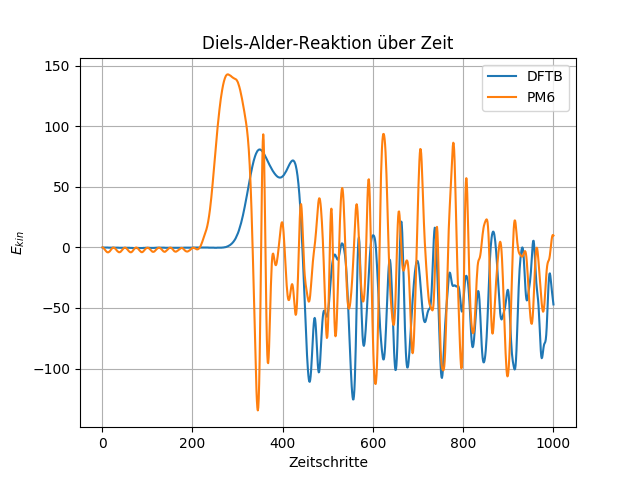
\includegraphics[scale=0.37]{dftb1_19pm61_57Data.png}
    \end{figure}
  \end{itemize}
\end{frame}
